\documentclass[12p, a4]{article}

\usepackage[T1]{fontenc}
\usepackage{lmodern}
\usepackage[ngerman]{babel}
\usepackage[utf8]{inputenc}
\usepackage{graphicx}

\title{The Embryonics Approach\\ \ \newline \ \newline - Zusammenfassung}
\author{Frank Lange}

\begin{document}

\begin{titlepage}
\title{The Embryonics Approach\\ \ \newline- Zusammenfassung -}
\author{Frank Lange}
\date{04. April 2013}
\maketitle
\thispagestyle{empty}
\end{titlepage}


\tableofcontents
\newpage





\section{Einleitung}
Grundsätzlich beschäftigt sich der ''Embryonic Approach'' mit Konzepten des
Designs und der Realisierung zukünftiger Generationen von integrierten
Schaltkreisen und versucht dabei, biologische Konzepte als Grundlage für
neue Ansätze zu benutzen. Im Folgenden sollen daher die aus [1] resultierenden
Ergebnisse zusammengefasst und vorgestellt werden.\\


\subsection{Motivation}
Die aktuelle Entwicklung von integrierten Schaltkreisen deutet darauf hin,
dass wir grundlegend neue Konzepte für den Schaltkreis Entwurf benötigen,
um auch in zukünftigen Generationen von integrierten Schaltkreisen eine
ähnliche Leistungssteigerung erreichen zu können, wie in den letzten
Jahrzehnten.\\
Ein absehbarer Trend ist dabei, dass die Verkleinerung des
Fertigungmaßstabes und damit auch einhergehend Moore's Law
höchstwahrscheinlich immer mehr stagnieren werden, da rein physikalisch
eine weitere Verkleinerung der aktuellen 22nm CMOS Transistortechnologie
kaum bis gar nicht möglich ist.\\
\ \newline
Es wird daher verstärkt nach neuen Konzepten gesucht, welche eine Fertigung
im nanoelektronischen Bereich in großer Anzahl erlauben. Dabei handelt es
sich nicht um den ''klassischen'' Fertigungsmaßstab im Nanometerbereich,
welcher jegliche Elektronik umfasst, die in einem kleineren Maßstab als 100nm
gefertigt wird, sondern meint einen Maßstab auf atomarer bzw. molekularer
Ebene, welcher also deutlich kleiner ist, als der aktuelle Stand der 22nm
Fertigung.\\


\subsection{Problemstellung}
Versucht man nun sich zukünftige Generationen integrierter Schaltkreise
im molekularen Maßstab vorzustellen, stößt man schnell auf Probleme,
die auch heute schon zu den aktuellen Problemen der Schaltkreisherstellung
gehören, welche allerdings mit einem imensen Faktor multipliziert werden,
sobald man den Herstellungsmaßstab nicht nur halbiert, sondern nun nochmals
um ein Vielfaches verkleinert.\\
\ \newline
Zum einen fällt allein die Anzahl der hergestellten Chips auf. Verringert
man den Fertigungsmaßstab erhöht man damit automatisch auch die Anzahl
der Chips, welche in ein und demselben physichen Raum hergestellt werden
können. Dabei stellt sich die Frage, wie man möglichst effizient möglichst
viele Chips herstellen kann, ohne dabei eventuell für jeden einzelnen den
gleichen Aufwand betreiben zu müssen, so wie es heute noch der Fall ist.\\
\ \newline
Zum anderen bewirkt eine Verkleinerung des Herstellungsmaßstabs auch eine
erhöhte Fehlerrate beim Herstellungsprozess. Dabei bieten sich zwei
mögliche Lösungsansätze intuitiv an. Man könnte entweder den
Herstellungsprozess so optimieren bzw. perfektionieren, sodass man die
Fehlerrate bei der Herstellung versucht auf ein Minimum zu reduzieren,
oder man versucht einen Fertigungsprozess zu entwerfen, welcher es den
hergestellten Chips erlaubt mit fehlerhaften Elementen möglichst tolerant
umzugehen.\\
\ \newline
Im folgenden sollen Konzepte zur Lösung beider Problemfälle vorgestellt und
erläutert werden. Dabei beschäftigt sich die Lösung des ersten Problemfalles
mit dem Konzept einer \textit{sich selbst vervielfältigender Hardware}.
Für den zweiten Problemfall wird mit Hilfe des Konzepts einer \textit{sich selbst
reparierenden Hardware} die Lösung mit erhöhter Fehlertoleranz vorgestellt.\\
In beiden Fällen dienen bestimmte biologische Konzepte der Natur als
Grundlage bzw. Ideengeber, welche zusätzlich an entsprechender Stelle mit
vorgestellt werden.
\ \newline




\section{Sich selbst vervielfältigende Hardware}
Im Folgenden soll das Konzept einer sich selbst heilenden Hardware
vorgestellt werden. Dabei bezieht sich der Begriff \textit{Hardware}
ausschließlich auf integrierte Schaltkreise.\\
Ziel ist es, dafür zu sorgen,
dass nur eine möglichst geringe Teilmenge von Schaltkreisen initialisiert
werden muss,
welche dann dafür sorgt, alle anderen Chips bei der Herstellung zu
initialisieren. Dabei werden \textit{1-zu-1 Klone} der Initialmenge von
\textit{von dieser selbst} erstellt. Dies soll dazu beitragen,
integrierte Schaltkreise in zukünftigen Generation effektiv in großen
Stückzahlen herstellen zu können.\\
\ \newline
Dabei ist die Grundlage des Konzepts die Art und Weise, wie in der Natur
mehrzellige Organismen intern organisiert sind und wie sie überhaupt
entstehen bzw. wachsen.\\


\subsection{Biologische Grundlage}
Betrachtet man die Art und Weise, wie mehrzelluläre Organismen aufgebaut sind,
so stellt man fest, dass sie aus einer endlichen Anzahl aus Zellen bestehen.
Jede dieser Zellen kann dabei einer größeren Gruppe wie z.B. Nervenzellen oder
Muskelzellen zugeordnet werden. Auf Grund dieser Zuordnung besitzt jede
Zelle eine charakteristische Funktion, welche sie ausübt, da sie z.B. die
Funktion als eine Muskelzelle übernimmt, wobei durchaus mehrere Zellen ein
und derselben funktionalen Gruppe zugeordnet werden.\\
Auffällig ist dabei,
dass die räumliche Position häufig ausschlaggebend für die übernommene
Funktionalität ist.\\
\ \newline
Es gibt allerdings auch eine bestimmte Menge an Zellen, welche (noch) keine
Funktionalität zugewiesen bekommen haben. Diese Zellen können zu einem
späteren Zeitpunkt, je nach Bedarf, eine beliebige Funktionalität
übernehmen bzw. ausprägen, was bei schon \textit{festgelegten} Zellen i.d.R.
nicht mehr möglich ist.\\
\ \newline
Mehrzelluläre Organismen \textit{wachsen} mit Hilfe des Vorgangs der
\textit{Zellteilung}. Dabei erstellt die Mutterzelle von sich selbst komplett
identische Klone, welche wiederum den Prozess der Zellteilung
einleiten und somit zu einem Wachstum des Organismus führen.\\


\subsection{Übetragung auf Schaltkreise}
Das aktuelle Konzept zur Übertragung dieser biologischen Konzepte auf den
Schaltkreisentwurf sieht dabei jetzt folgendes vor.\\Jede \textit{Zelle}
ist ein kleiner Mikroprozessor mit einer geringen Menge Arbeitsspeicher und
befindet sich, wie bei der Massenherstellung von integrierten Schaltkreisen
üblich, in einem Grid von solchen.
Dieses Grid wäre vollständig initialisiert, wenn jede Zelle des Grids in
ihrem Arbeitsspeicher das komplette \textit{Programm} besäße und an Hand
ihrer eigenen Position/Koordinate innerhalb des Grids wüsste, welchen
Teil des Programms sie ausführen soll. Dabei wäre dieses \textit{globale
Programm} das Pendent zum biologischen Genom.\\


\subsection{Zellen und Organismen}
Um also nun ein gesamtes Grid von intialisierten Zellen zu erhalten, würde es
ausreichen, nur eine initiale Menge von Zellen mit dem \textit{Genom} und
ihren Koordinaten auszustatten und dafür zu sorgen, dass noch uninitialisierte
Zellen das \textit{Genom} in ihren Arbeitsspeicher kopiert und dann
eine Koordinate zugewiesen bekommen, an Hand derer sie ableiten können,
welchen Teil des Genoms sie \textit{anspringen}, d.h. ausführen sollen.\\
\ \newline
Mit Hilfe der Modulo-Funktion bei der Berechnung einer Koordinate einer noch
uninitialisierten Zelle wird sichergestellt, dass sich im Laufe der Zeit
auf dem gesamten Grid ein sich stets wiederholendes Pattern erkennbar wird.
Solch ein \textit{Pattern} wird dabei als ein \textit{Organismus}
aufgefasst, da alle zu einem \textit{Organismus} gehörigen Zellen auf Grund
ihrer paarweise verschiedenen Koordinaten (innerhalb des Organismus) jeweils
einen anderen Teil des Genoms und somit als Kollektiv das gesamte
Genom ausführen.\\
\ \newline
Auf dem gesamten Grid befinden sich dann also letztendlich nach einigen Zyklen
Zellen, welche vorher uninitialisert waren und welche nun nicht
nur eine Koordinate zugewiesen bekommen haben und einen bestimmten Teil des
Gesamtgenoms ausführen, sondern welche auch mit angrenzenden Zellen unbewusst
als Kollektiv arbeiten und somit gedacht einen Organismus darstellen. Wobei
das Gesamte Grid dann aus Organismenklonen der ursprünglichen Initialmenge von
Zellen, d.h. dem ursprünglichen Organismus besteht (Abb. 1).\\
\ \newline
\begin{figure}[h]
  \centering
    \includegraphics[width=\linewidth]{cell_coords2.png}
  \caption{Mehrere Kopien eines Organimus in einem Zellgrid}
  \label{}
\end{figure}

\subsection{Moleküle}
Um solch ein Propagieren von Genom und Koordinate möglich zu machen
besteht, sowie ein gedachter Organismus aus mehreren gedachten Zellen besteht,
auch eine Zelle aus mehrere sog. \textit{Molekülen}. Wobei es sich bei
Molekülen nicht mehr um konzeptionelle Gebilde handelt sondern diese aus
einem oder mehreren \textit{Field Programmable Gate Arrays} (FPGA) bestehen,
d.h. aus wirklichen Schaltkreiselementen.\\
\ \newline
Das besondere an FPGAs ist, das diese über eine Schaltungstabelle verfügen,
über welche, durch das Anlegen bestimmter Eingangsbelegungen, die Funktion
des FPGAs bestimmt wird. Das bedeutet man kann die Funktionalität dieses
Schaltkreiselements durch das Anlegen bestimmter Eingangsbelegungen auch
''zur Laufzeit'' ändern.\\
\ \newline
Das Besondere ist nun, dass das Grid aus den gedachten \textit{Zellen}
im Grunde nur ein Grid aus solchen FPGAs ist, wobei jeweils die Ausgänge
eines FPGAs als die Eingänge eines weiteren FPGAs benutzt werden, wodurch
Informationen über die Funktionalität von einem FPGA zum nächsten propagiert
werden können.\\
\ \newline
Damit also nun Informationen bzw. Abarbeitungsbefehle von einem FPGA zum
Nächsten, d.h. von einem Molekül zum Nächsten weitergegeben werden können,
werden bestimmte Befehle benötigt, die angeben, in welche Richtung bzw.
an welche Ausgänge die Informationen weitergeleitet werden sollen.
Das bedeutet, man muss zu Beginn ganz genau überlegen, welche Befehlsfolge
zum einen dafür sorgt, dass jedes Molekühl einer Zelle eine Funktionalität
zugeordnet bekommt, zum anderen aber jedes Molekül bestimmte Befehle auch
weitergibt, sodass anliegende Moleküle, welche noch nicht
initialisiert/programmiert wurden sozusagen ''aktiviert'' bzw. initialisiert
werden.\\
\ \newline
Im Endeffekt reicht eine sorgsam erstellte Befehlsfolge von wenigen Befehlen
aus, um eine Verbreitung dieser Befehle über das gesamte Grid zu bewirken.\\


\section{Sich selbst reparierende Hardware}
Nachdem bisher das erste Konzept einer sich selbst vervielfältigen Hardware
vorgestellt wurde, soll im folgenden das Konzept einer sich selbst
reparierenden Hardware vorgestellt und genau erläutert werden.\\
Auch hier bezieht sich der Begriff \textit{Hardware} ausschließlich auf
integrierte Schaltkreise.\\
\ \newline
Ziel dieses Konzept ist es, die Fehlertoleranz
zukünftiger Generationen integrierter Schaltkreise zu erhöhen.\\


\subsection{Biologische Grundlage}
Wie schon beim Konzept einer sich selbst vervielfältigen Hardware sind auch
hier wieder biologische Konzepte die Ideengeber. Wo vorher allerdings
mehrzelluläre Organismen als solche betrachtet wurden, ist an dieser Stelle
interessanter, mit welcher Art und Weise eine Spezies für ihr Überleben sorgt.
Dabei ist der wichtigste Faktor der, der Redundanz.\\
\ \newline
Wenn man eine beliebige Population einer Spezies betrachtet, so stellt
man fest, dass diese Population zwar aus mehreren individuellen und
unabhängigen Organismen besteht, diese allerdings alle die gesamte und somit
alle die gleiche Erbinformation der Spezies in sich tragen. Das bedeutet
logischer Weise, dass die Spezies existiert, solange ein Individuum existiert.
Alle anderen Individuen sind, wenn auch etwas drastisch formuliert,
Redundanz, um eventuellen Ausfällen einzelner Organismen vorzubeugen.\\
\ \newline
Genau so bestehen wiederum einzelne Organismen dieser Population aus Zellen,
wobei jede Zelle die komplette Erbinformation des Organismus in sich trägt.
Erst wenn man noch ein weiteres mal rekursiv Absteigt findet man zwar, dass
die Zelle wiederum aus einzelnen Molekülen besteht, diese jedoch keine
weitere Redundanz bieten. Man ist also an der Basis angekommen.\\
\ \newline
Das bedeutet nun also, dass die Natur nicht versucht ihren
Fortpflanzungsprozess zu perfektionieren und damit Mutationen auszuklammern,
sondern vielmehr, dass sie mit Fehlertoleranz in Form von Redundanz einen
Weg gefunden hat, mit einer permanten Fehlerrate erfolgreich umzugehen.\\
\ \newline
\begin{figure}[h]
  \centering
    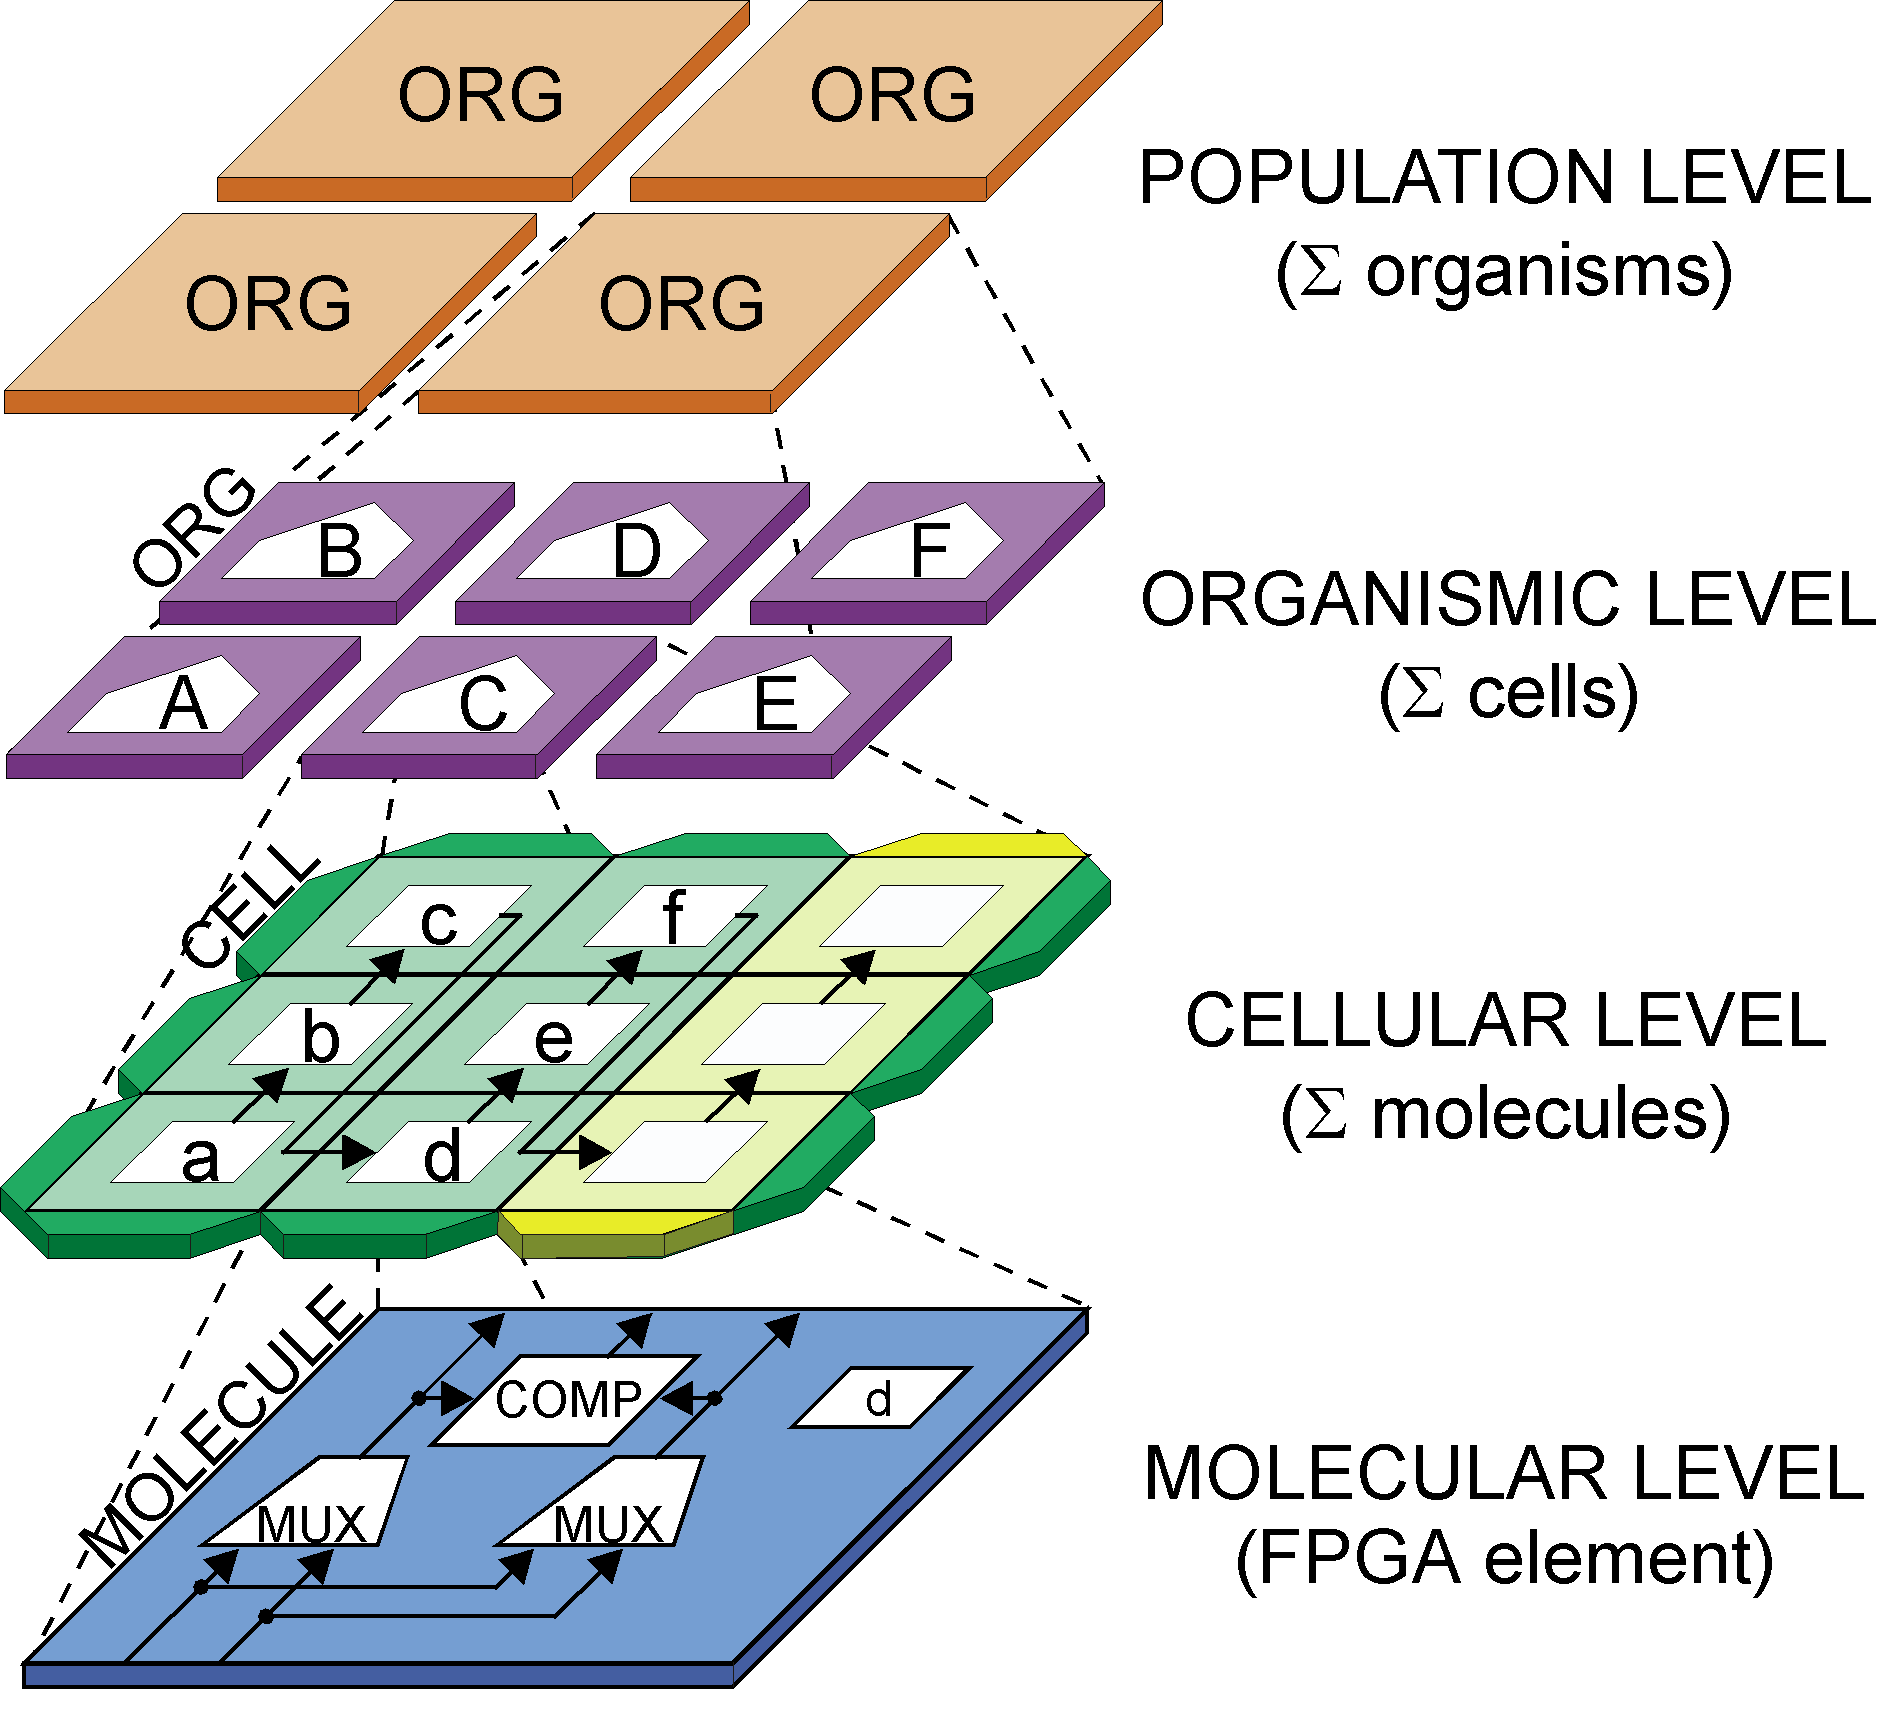
\includegraphics[width=\linewidth]{4level.png}
  \caption{Konzept der einzelnen Ebenen}
  \label{}
\end{figure}
\subsection{Übertragung auf Schaltkreise}
Übertragt man diese Idee der mehrschichtigen Redundanz nun auf den
Schaltkreisentwurf, bietet es sich an, mit den schon oben eingeführten
Konzepten wie Molekülen, Zellen und Organismen weiterzuarbeiten, wobei auch
hier ein gedachtes Molekül aus einem FPGA besteht und eine Zelle einen aus
mehrere Molekülen bestehender Mikroprozessor inklusive Speicher und ein
Organismus einen aus mehreren Zellen bestehenden ''Mehrkern''-Prozessor
darstellt (Abb. 2).\\
\ \newline
Diesmal auf der Ebene der Moleküle beginnend stellt man fest, dass es für
einen Produktionsfehler/Ausfall eines FPGAs keine Möglichkeit gibt, diesen
im Nachhinein zu korrigieren. Die einzige Möglichkeit die sich an dieser
Stelle anbietet, ist es, das kaputte Molekül mit einem funktionierenden
Molekül zu ersetzen. Dafür ist es nötig, Moleküle zu haben, welche im
Normalfall keine Funktionalität besitzen, sondern nur als Ersatzmoleküle
für einen Fehlerfall dienen.\\
\ \newline
Das gute ist dabei, dass die Anzahl dieser Ersatzmoleküle variable
bestimmt werden kann, da beim Initialisieren des Grids wie
im Abschnitt 2 (s.o.) in der verwendeten Befehlsfolge nur dafür gesorgt werden
muss,
dass bestimmte Moleküle bzw. Zellen keine Funktionalität erhalten, sondern
erhaltene Informationen ersteinmal nur weiterleiten. Somit kann man die
Fehlertoleranz des Systems je nach Einsatzgebiet passend wählen.\\
\ \newline
Sollte ein Molekül also ausfallen, werden seine Registerinhalte innerhalb
der Zelle des Moleküls zu seinem
rechten Nachbar transferiert. Sollte es sich dabei nicht um ein
Ersatzmolekül handeln, gibt auch diese Molekül seine Registerinhalte zu seinem
rechten Nachbar weiter, solange bis innerhalb der Zelle ein Ersatzmolekül
erreicht wird. Sollte kein Ersatzmolekül innerhalb der Zelle verfügbar sein,
wird der Reparationsmechanismus auf der nächsthöheren, also der zellulären
Ebene aktiviert.\\
\ \newline
Sollte ein Fehler auf molekularer Ebene nicht behandelbar sein, wird an
die betroffene Zelle ein sog. ''KILL''-Signal gesendet. Dieses bewirkt,
dass die betroffene Zelle, oder der Einfachheit der Realisierung halber,
die gesamte Spalte von Zellen stirbt.\\
Auf der zellulären Ebene bedeutet dies, dass auch hier die Inhalte der
betroffenen Zellen zu ihrem rechten Nachbarn transferiert werden, bis
eine Spalte von Ersatzzellen erreicht wird. Danach werden die betroffenen
Zellen als tot markiert und jeglicher Informationstransfer in Zukunft
um diese Zellen herum geleitet. Desweiteren müssen in diesem Falle alle
Koordinaten der Zellen innerhalb des betroffenen Organismus neu berechnet
bzw. neu bestimmt werden.\\





\section{Zusammenfassung}
Nachdem die Konzepte einer sich selbst vervielfältigenden und einer sich
selbst reparierenden Hardware vorgestellt und erläutert wurden, sollen im
Folgenden nochmal die Eckpunkte der beiden Konzepte zusammengefasst und
ein Überblick über die Erfüllung der Anforderungen an diese beiden Konzepte
gegeben werden. Dabei sei darauf hingewiesen, dass auch, wenn diese beiden
Konzepte in dieser Arbeit getrennt vorgestellt und behandelt wurden, sie
doch eine gemeinsame Symbiose darstellen und für den kollektiven Einsatz
gedacht sind.\\


\subsection{Selbst reparierende Hardware}
Das in Abschnitt 3 vorgestellte Konzept einer sich selbst reparierenden bzw.
selbst heilenden Hardware in Bezug auf integrierte Schaltkreise biete einige
Denkansätze, welche in Zukunft mit Sicherheit weiter ausgebaut werden.\\
\ \newline
Die wichtigsten Eigenschaften dieses Konzepts und der damit verbundenen
Verfahren sind sicherlich, dass die erreichte Fehlertoleranz des Systems
nicht nur auf einer Ebene oder an einer bestimmten Stelle vorhanden ist,
sondern sich, wie im natürlich Vorbild, durch mehrere Ebenen zieht.
Dadurch wird erreicht, dass die ''Reparatur'' nicht über einen zentralen
Kontrollmechanismus gesteuert werden muss, sondern so lokal wie nur möglich
erfolgen kann.\\
\ \newline
Die große Einschränkung besteht allerdings darin, dass eine wirkliche
Reparatur auf Molekülebene, also auf FPGA Ebene, unrealistisch ist und somit
nicht erfolgen kann. Dass bedeutet, die eigentliche \textit{Reparatur} wird
Verlagert in ein \textit{Ersetzen} fehlerbehafteter Moleküle.\\
\ \newline
Ob nun, bei immer kleiner werdendem Fertigungsmaßstab, auch die Anzahl der
Erzahlmoleküle in einer solcher Form steigt, dass sich Vorteile des
kleineren Fertigungsmaßstab und der Nachteil der dann benötigten
Ersatzmoleküle relativieren, bleibt zur Zeit ungeklärt.


\subsection{Selbst vervielfältigende Hardware}
Das in Abschnitt 2 vorgestellte Konzept einer sich selbst vervielfältigenden
Hardware in Bezug auf den Entwurf integrierter Schaltkreise bildet
die eigentliche Grundlage der beiden hier vorgestellten Konzepte, da es
sich im Kern auf der Informationsfortpflanzung zwischen FPGAs stützt.\\
\ \newline
Die Idee, eine große Menge an Chips nur mit einer Initialaktion sich selbst
programmieren zu lassen, wird von diesem Konzept vollständig umschlossen.
Die Schwächen des Konzepts liegen aber vor allem darin, dass es kein
Konzept zur eigentlichen Herstellung von integrierten Schaltkreisen liefert,
da es sich ausschließlich in einem schon vorbereiteten, d.h. schon erstellten
Grid von FPGAs ausbreiten und diese schon vorhandenen Elemente programmieren
kann. Hinzukommt, dass alle von dem Konzepten erzeugten Schaltkreisorganismen
identische Klone des Ausgangsorganismus sind, da eine Abbildung des
natürlichen Konzepts der Mutation, z.Z. auf FPGA Ebene noch nicht möglich
ist.\\
\ \newpage

\section{Quellen}
[1] G. Tempesti, D. Mange, A- Stauffer, "Bio-Inspired Computing\\
Architectures:
The Embryonics Approach", in Proceedings of the Seventh International
Workshop on Computer Architecture for Machine Perception (CAMP’05)\newline
[Online]: http://www-users.york.ac.uk/~gt512/Publications/2005/CAMP05-Tempesti.pdf\\
\ \newline
Abbildung 1:\\
http://lslwww.epfl.ch/pages/embryonics/thesis/Thesis-11.gif\\
\ \newline
Abbildung 2:\\
http://www-users.york.ac.uk/ gt512/Images/4Level.gif\\
\ \newline



\end{document}
